\section{Literaturrecherche} \label{literaturrecherche}

Um einen Überblick über den aktuellen Stand der Forschung zu bekommen wird zunächst eine Literaturrecherche vorgenommen. Dabei sollen vorhandene online IDEs gefunden sowie die folgenden Fragen beantwortet werden:

\begin{itemize}
    \item Welche Implementierungen von online IDEs gibt es?
    \item Welchen Architekturmustern folgen online IDEs?
    \item Welche Vor- und Nachteile haben die online IDEs?
    \item Welche Anforderungen werden an online IDEs gestellt?
\end{itemize}

Die folgenden Datenbanken wurden für die Literaturrecherche ausgewählt:

\begin{itemize}
    \item ACM Digital Library
    \item IEEE Xplore
    \item Scopus
    \item Web of Science
\end{itemize}

Zunächst wurde eine allgemeine Suche nach online IDEs in den genannten Datenbanken vorgenommen. Dazu werden zunächst die in Tabelle \ref{table:search-terms} genannten Stichwörter jeweils mit ihren Synonymen mit einer OR-Operation verknüpft. Danach werden die daraus resultierenden Terme mit einer AND-Operation verbunden. Die so entstehende Suchanfrage werden dann für die Suche in den Datenbanken verwendet. Dabei werden die Titel, Abstracts und Keywords der Publikationen durchsucht.

In Tabelle \ref{table:amount-search-results} ist die Anzahl der Treffer für den einzelnen Datenbanken dargelegt. Um die Anzahl der zu betrachtenden Publikationen zu verringern wird eine weitere Filterung der Ergebnisse vorgenommen. Dafür werden nur Publikationen betrachtet, die IDE oder ein entsprechendes Synonym in ihrem Titel oder ihren Keywords enthalten. Dadurch sinkt die Anzahl der Treffer auf insgesamt $1705$. Danach werden alle exakten Duplikate über einen Vergleich der Titel und Links herausgefiltert wodurch die Anzahl der Publikationen auf $1243$ sinkt. In einem weiteren Schritt werden die Titel und Abstracts der Publikationen genauer betrachtet. Dabei werden unter anderem Arbeiten herausgefiltert, deren Titel und Abstracts keinen Bezug zu den Forschungsfragen besitzen. Weiterhin werden Publikationen bevorzugt, die sich zudem mit textbasierten Programmiersprachen, Kollaboration und Lehre auf Universitätsniveau befassen. Aus dieser Filterung resultieren $97$ Publikationen. Als letzte Filterung werden Publikationen, welche vor $2019$ veröffentlicht wurden aussortiert, falls sie weniger als $10$ Zitationen haben sowie vor $2014$ veröffentlichte Publikationen mit weniger als $25$ Zitationen. Die Anzahl der Zitationen wurde mithilfe von Google Scholar ermittelt. Dadurch ergibt sich die Anzahl von $64$ zu betrachtenden Publikationen.

\begin{table}[tbp]
    \centering
    \begin{tabularx}{\textwidth}{| >{\hsize=.6\hsize\linewidth=\hsize}X |
            >{\hsize=1.4\hsize\linewidth=\hsize}X |}
        \hline
        Stichwort                           & Synonyme                                                                                                     \\
        \hline
        integrated development environments & IDEs, code editors, development environments, development tools, programming tools, programming environments \\
        \hline
        web                                 & browser, online, cloud                                                                                       \\
        \hline
    \end{tabularx}
    \caption{Suchbegriffe}
    \label{table:search-terms}
\end{table}

\begin{table}[tbp]
    \centering
    \begin{tabular}{|c|c|c|c|c|c|}
        \hline
        ACM & IEEE & Scopus & Web of Science \\
        \hline
        785 & 1472 & 4661   & 1044           \\
        \hline
    \end{tabular}
    \caption{Anzahl Suchergebnisse}
    \label{table:amount-search-results}
\end{table}

\begin{figure}[htbp]
    \centering
    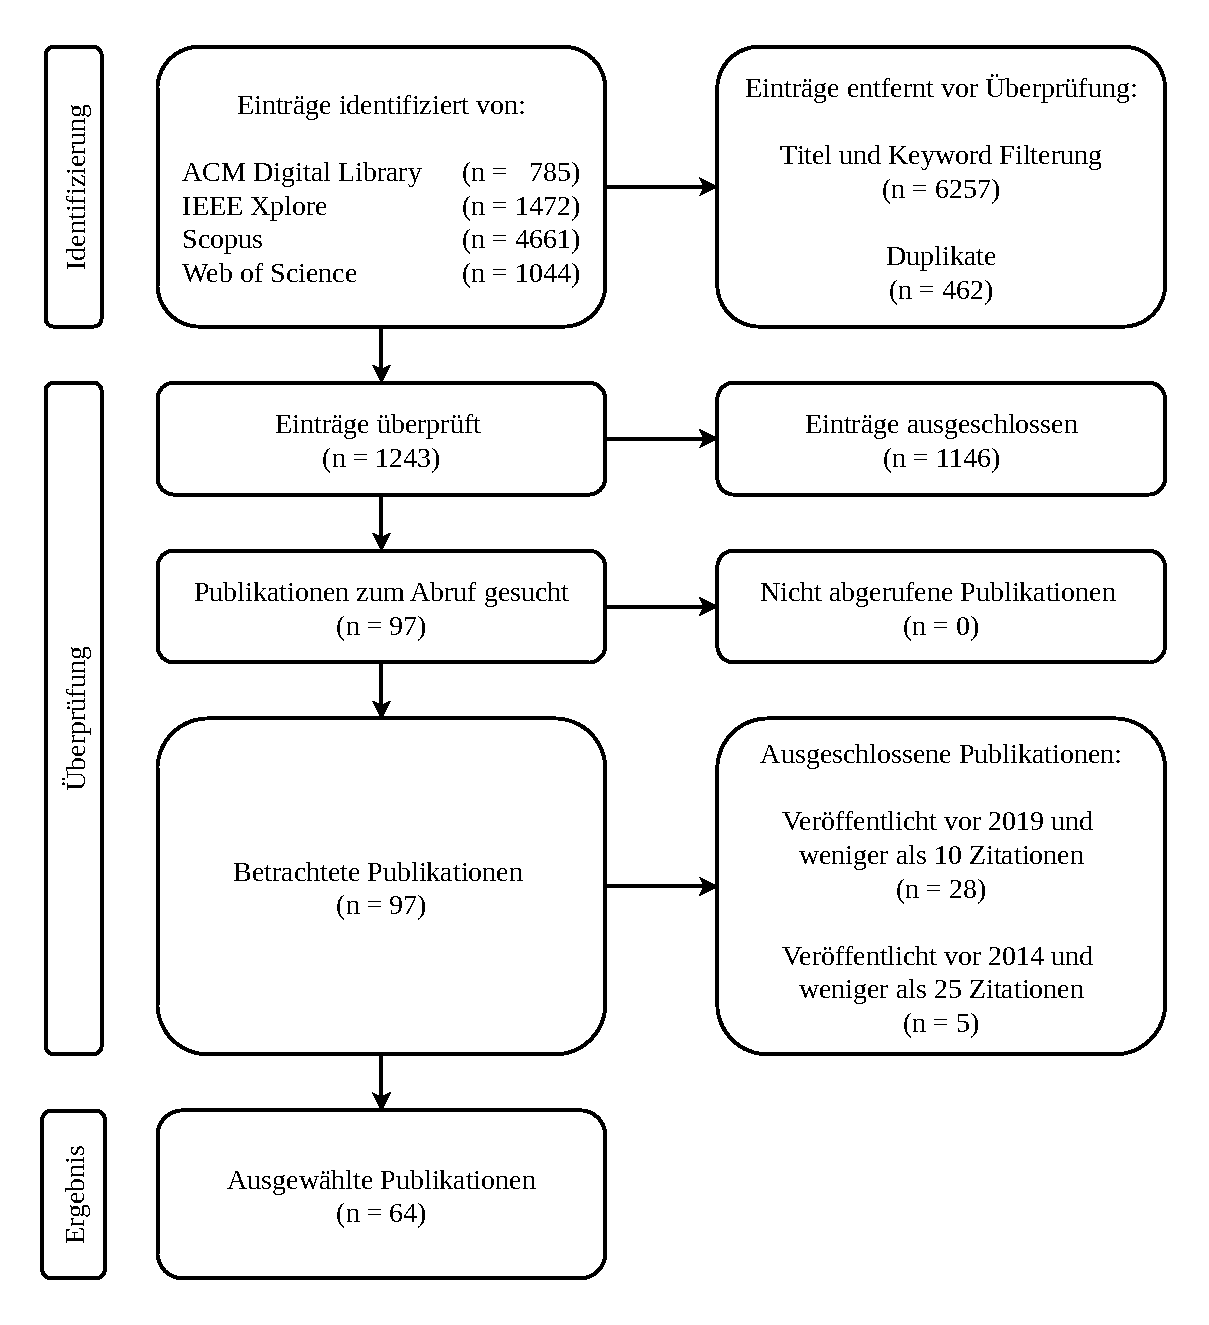
\includegraphics[width=\textwidth]{diagrams/PRISMA.pdf}
    \caption{PRISMA Diagramm}
    \label{prisma-diagram}
\end{figure}

Die Publikationen beschreiben eine Vielzahl an verschiedenen webbasierten integrierten Entwicklungsumgebungen. Dabei kann eine Unterteilung in die folgenden zwei Kategorien erfolgen:

\begin{itemize}
    \item \textbf{Client-Server-basierte Lösungen} \\
          Systeme dieser Art zeichnen sich dadurch aus, dass sie eine Client-Server-Archi-tektur verwenden. Hierbei werden Features, die nicht innerhalb eines Browsers ausgeführt werden können (z.B. Kompilierung) über einen entsprechenden Server bereitgestellt.
    \item \textbf{Browser-basierte Lösungen} \\
          Systeme dieser Art zeichnen sich dadurch aus, dass alle Features im Browser des Nutzers ausgeführt werden können, ohne die Hilfe eines separaten Servers.
\end{itemize}

Deursen et al. (2010) \cite{van_deursen_adinda_2010} beschreiben eine online IDE names Adinda. Die grundlegende Idee von Adinda ist die Zerlegung der Funktionalität einer IDE in einen leichtgewichtigen Client sowie mehrere zusammenarbeitende (Web-)Services. Diese Services sollen dann bestimmte Aufgaben erfüllen, wie z.B. Kompilierung, Testen, kollaboratives Editieren und Datenerhebung. Es werden weiterhin verschiedenste Forschungsfragen aufgestellt, die für das vorgestellte System von Interesse sind. Die prototypische Implementierung von Adinda basiert auf WWWorkspace \cite{ryan_web_2007} und nutzt serverseitig Eclipse \cite{noauthor_eclipse_nodate}. Der Prototyp unterstützt das Erstellen von Nutzer-Workspaces, Java Projekten, Paketen und Klassendateien sowie Syntax Highlighting, Kompilierung und Code-Vervollständigung. \todo{Adinda} \\

Wu et al. (2011) \cite{wu_ceclipse_2011} stellen die online IDE Cloud Eclipse (CEclipse) vor. Die Ziele von CEclipse sind:
\begin{enumerate}
    \item die Bereitstellung von Eclipse \cite{noauthor_eclipse_nodate} Funktionen wie z.B. Code-Vervollständigung
    \item die Behandlung von den online IDE spezifischen Sicherheitsproblemen \quoted{\textit{Wrong file operations}}, \quoted{\textit{Banned operation calling}} und \quoted{\textit{Excessive resource consumption}}
    \item die Ausnutzung von Cloud Computing Möglichkeiten um Entwickler besser zu unterstützen.
\end{enumerate} 
Für $1.$ wurde ein entsprechendes Protokoll entwickelt, was es ermöglicht die gewünschten Funktionen von Eclipse aufzurufen und das Ergebnis im Browser darzustellen. Um die in $2.$ genannten Probleme Handhaben zu können wird ein \textit{Program Behavior Analysis Service} beschrieben. Durch die Einschränkung des Dateisystems auf einen speziellen Ordner kann das Problem \quoted{Wrong file operations} gelöst werden. Das Verbieten bzw. Erlauben von Methoden über eine Blacklist bzw. eine Whitelist kann zur Lösung des Problems \quoted{Banned operation calling} angewendet werden. Durch eine Zeitbegrenzung von laufenden Prozessen kann schließlich auch das Problem \quoted{Excessive resource consumption} behoben werden. Für $3.$ werden über den \textit{Program Behavior Mining Service} Daten über die Nutzung der IDE gesammelt werden. Diese Daten können dann z.B. dazu genutzt werden dem Entwickler häufig verwendete Befehle mit höherer Priorität vorzuschlagen. \todo{CEclipse} \\

Goldman et al. (2011) \cite{goldman_real-time_2011} beschreiben Collabode, eine kollaborative online IDE für Java. Collabode ermöglicht es mehreren Nutzern gleichzeitig Änderungen an Dateien vorzunehmen. Die Änderungen werden in Echtzeit zwischen den Nutzern synchronisiert. Dabei wird ein spezieller Algorithmus verwendet. Dieser Algorithmus sorgt dafür, dass nur Änderungen eingepflegt werden, die keinen syntaktischen Fehler beinhalten oder erzeugen. Dadurch wird sichergestellt, das Nutzer nur ihre eigenen Fehler sehen und das Programm unabhängig von den ggf. vorhandenen Fehlern ihrer Teammitglieder kompilieren können. Collabode nutzt EtherPad \cite{noauthor_etherpad_nodate} als Editor im Frontend und Eclipse \cite{noauthor_eclipse_nodate} für die Bereitstellung von Kompilierung, Syntax Highlighting, etc. im Backend. \todo{Collabode} \\

Lautamäki et al. (2012) \cite{lautamaki_cored_2012} stellen Collaborative Real-time Editor (CoRED) vor, einen online Code Editor für Java Programme. CoRED nutzt den ACE Editor \cite{noauthor_ace_nodate} im Fronted sowie das Java Development Kit (JDK) \todoaddref[]{JDK} zur Kompilierung im Backend. Fehlermeldungen während des Kompiliervorgangs werden an den Client zurückgesendet und dann im Frontend visualisiert. Zur Bereitstellung von Echtzeit Kollaboration wird der Algorithmus \textit{Differential Synchronization with shadows} \cite{fraser_differential_2009} von Neil Fraser eingesetzt. Ein weiteres Feature von CoRED ist das Sperren von Code Bereichen für andere Nutzer sowie die Möglichkeit Kommentare im Code zu hinterlassen. Auf diese Kommentare können dann andere Nutzer antworten, wodurch eine weitere Interaktionsmöglichkeit besteht. Weiterhin bietet CoRED auch Code-Vervollständigung an. \todo{CoRED} \\

Ball et al. (2015) \cite{ball_beyond_2015} beschreiben TouchDevelop. TouchDevelop ist eine online IDE bzw. eine cloudbasierte IDE (CIDE). Das Hauptfeature von TouchDevelop ist die Speicherung aller Programmänderungen, Versionen, Laufzeitinformationen, Bugs sowie Kommentare, Fragen und Feedback von Nutzern in einer zentralen Datenbank. Diese Daten können über entsprechende APIs abgefragt werden. Die Nutzeroberfläche von TouchDevelop unterscheidet sich stark von anderen textbasierten Editoren. So bekommt der Nutzer eine Auswahl an kontextabhängigen Optionen, z.B. if-Anweisungen, for-Schleifen oder verfügbare Variablen. Alle IDE Funktionen sind offline verfügbar, da sie komplett auf der Clientseite implementiert sind. Weiterhin nutzt TouchDevelop eine eigene Programmiersprache. Diese folgt dem imperativen Programmierparadigma, besitzt ein starkes Typsystem sowie eine Vielzahl an plattformübergreifenden APIs. \dots \todo{TouchDevelop} \\

Tran et al. (2013) \cite{tran_interactive_2013} \dots \\
Nguyen et al. (2014) \cite{nguyen_learning_2014} \dots \\
Nguyen et al. (2016) \cite{nguyen_enhancing_2016} \dots \todo{IDEOL/EduCo} \\

Warner und Guo (2017) \cite{warner_codepilot_2017} \dots \todo{CodePilot} \\

Über mehrere Publikationen wird die Entwicklung der Reflex IDE (RIDE) beschrieben.  Zunächst wird von Bastrykina et al. (2021) \cite{bastrykina_developing_2021} ein entsprechender Kernel mit dem Xtext Framework \cite{noauthor_xtext_nodate} entwickelt, welcher in der Eclipse IDE verwendet werden kann, um diese \todo{}. Darauf aufbauend wird von Gornev und Liakh (2021) \cite{gornev_ride_2021} die Konzipierung und Implementierung einer auf Theia basierten Web-Variante von RIDE vorgestellt. Gornev et al. (2022) \cite{gornev_towards_2022} beschreiben ein System, welches Docker verwendet um die Web-Version von RIDE für mehrere simultane Nutzer bereitstellen zu können. Gornev und Bondarchuk (2023) \cite{gornev_towards_2023} entwickeln ein Framework, welches es erlaubt Echtzeit-Kollaboration in Single-User Anwendungen zu ermöglichen. Kuznetsov und Zyubin (2024) \cite{kuznetsov_development_2024} beschreiben die Entwicklung eines Projektmanagement-Systems für RIDE. \todo{RIDE} \\

Jefferson et al. (2024) \cite{jefferson_pyodideu_2024} beschreiben eine IDE, die es Nutzern ermöglicht Python Code im Browser zu schreiben und auszuführen. Dabei wird das Programm des Nutzers lokal in dessem Browser durchgeführt. Dies wird durch den Einsatz von PyodideU erreicht, einer erweiterten Version der WebAssembly-basierten Python Distribution Pyodide \cite{noauthor_pyodide_nodate}. Zusätzlich wird den Nutzern auch eine Grafikbibliothek angeboten samt eines Debuggers, der es ermöglicht Zeile für Zeile und auch rückwärts durch das Programm zu gehen und die entsprechenden Änderungen an der Grafik zu sehen. Weiterhin wird durch PyodideU auch die synchrone Eingabe von Daten unterstützt, während Python im Main-Thread des Browsers läuft. Zudem wird auch ein Dateisystem bereitgestellt. Insgesamt wurde die IDE sowohl von Studenten als auch von Lehrenden als hilfreich wahrgenommen. \todo{PyodideU} \\

Malan (2024) \cite{malan_containerizing_2024} beschreibt die verschiedenen Ansätze zur Bereitstellung einer integrierten Entwicklungsumgebung für die Teilnehmer des Einführungskurses in die Programmierung (CS50) an der Harvard University. Zunächst wurde seit 2007 ein On-Campus Cluster für die Studenten angeboten. Studenten konnten über SSH mit diesem verbinden und dort ihre Programme ausführen. Dieser Cluster wurde 2008 mithilfe von Amazon Web Services (AWS) \cite{noauthor_amazon_nodate} in die Cloud überführt. Diese cloud-basierte Lösung wurde 2011 durch Client-seitige virtuelle Maschinen ersetzt. In 2015 wurde eine auf Docker basierende Lösung erarbeitet, die zunächst Cloud9 IDE \cite{noauthor_cloud_nodate} als Frontend nutzte. In 2021 wurde schlielich eine auf Github Codespaces aufbauende Lösung eingeführt, die VSCode als Code Editor verwendet. \todo{CS50} \\

\todo{Vorteile von online IDEs}

\todo{Nachteile von online IDEs}

\todo{Anforderungen an online IDEs}